% Editable article source. Builds never regenerate this file from Markdown.
\documentclass[11pt,letterpaper]{article}
\usepackage[margin=0.8in]{geometry}
\usepackage[T1]{fontenc}
\usepackage[utf8]{inputenc}
\usepackage{lmodern,microtype,amsmath,amssymb,graphicx}
\usepackage{booktabs,longtable,array,caption,parskip}
\usepackage[numbers,sort&compress]{natbib}
\usepackage{xurl}
\usepackage[colorlinks=true,linkcolor=blue,citecolor=blue,urlcolor=blue]{hyperref}
\setlength{\emergencystretch}{2em}
\setlength{\LTpre}{6pt}\setlength{\LTpost}{8pt}
\renewcommand{\arraystretch}{1.13}
\captionsetup{font=small,labelfont=bf,hypcap=false}
\newcolumntype{L}[1]{>{\raggedright\arraybackslash}p{#1}}
\newcommand{\dox}{\operatorname{do}}
\title{From a Plausible DAG to Causal Attribution\\[5pt]\large A Method Playbook for the Spaceflight Study}
\author{Working guide aligned with the manuscript's 13-step protocol}
\date{16 September 2026}
\makeatletter
\renewcommand{\maketitle}{\begin{center}{\LARGE\bfseries\@title\par}\vspace{7pt}\@author\\\@date\end{center}\vspace{3pt}}
\makeatother
\begin{document}
\maketitle

This playbook follows the study's method sequence: prepare the data and predictive reference, optionally discover structure, review the graph, define interventions, calculate causal attributions, and compare the results under specified data constraints. The goal gate determines which parts are needed.

\begin{center}
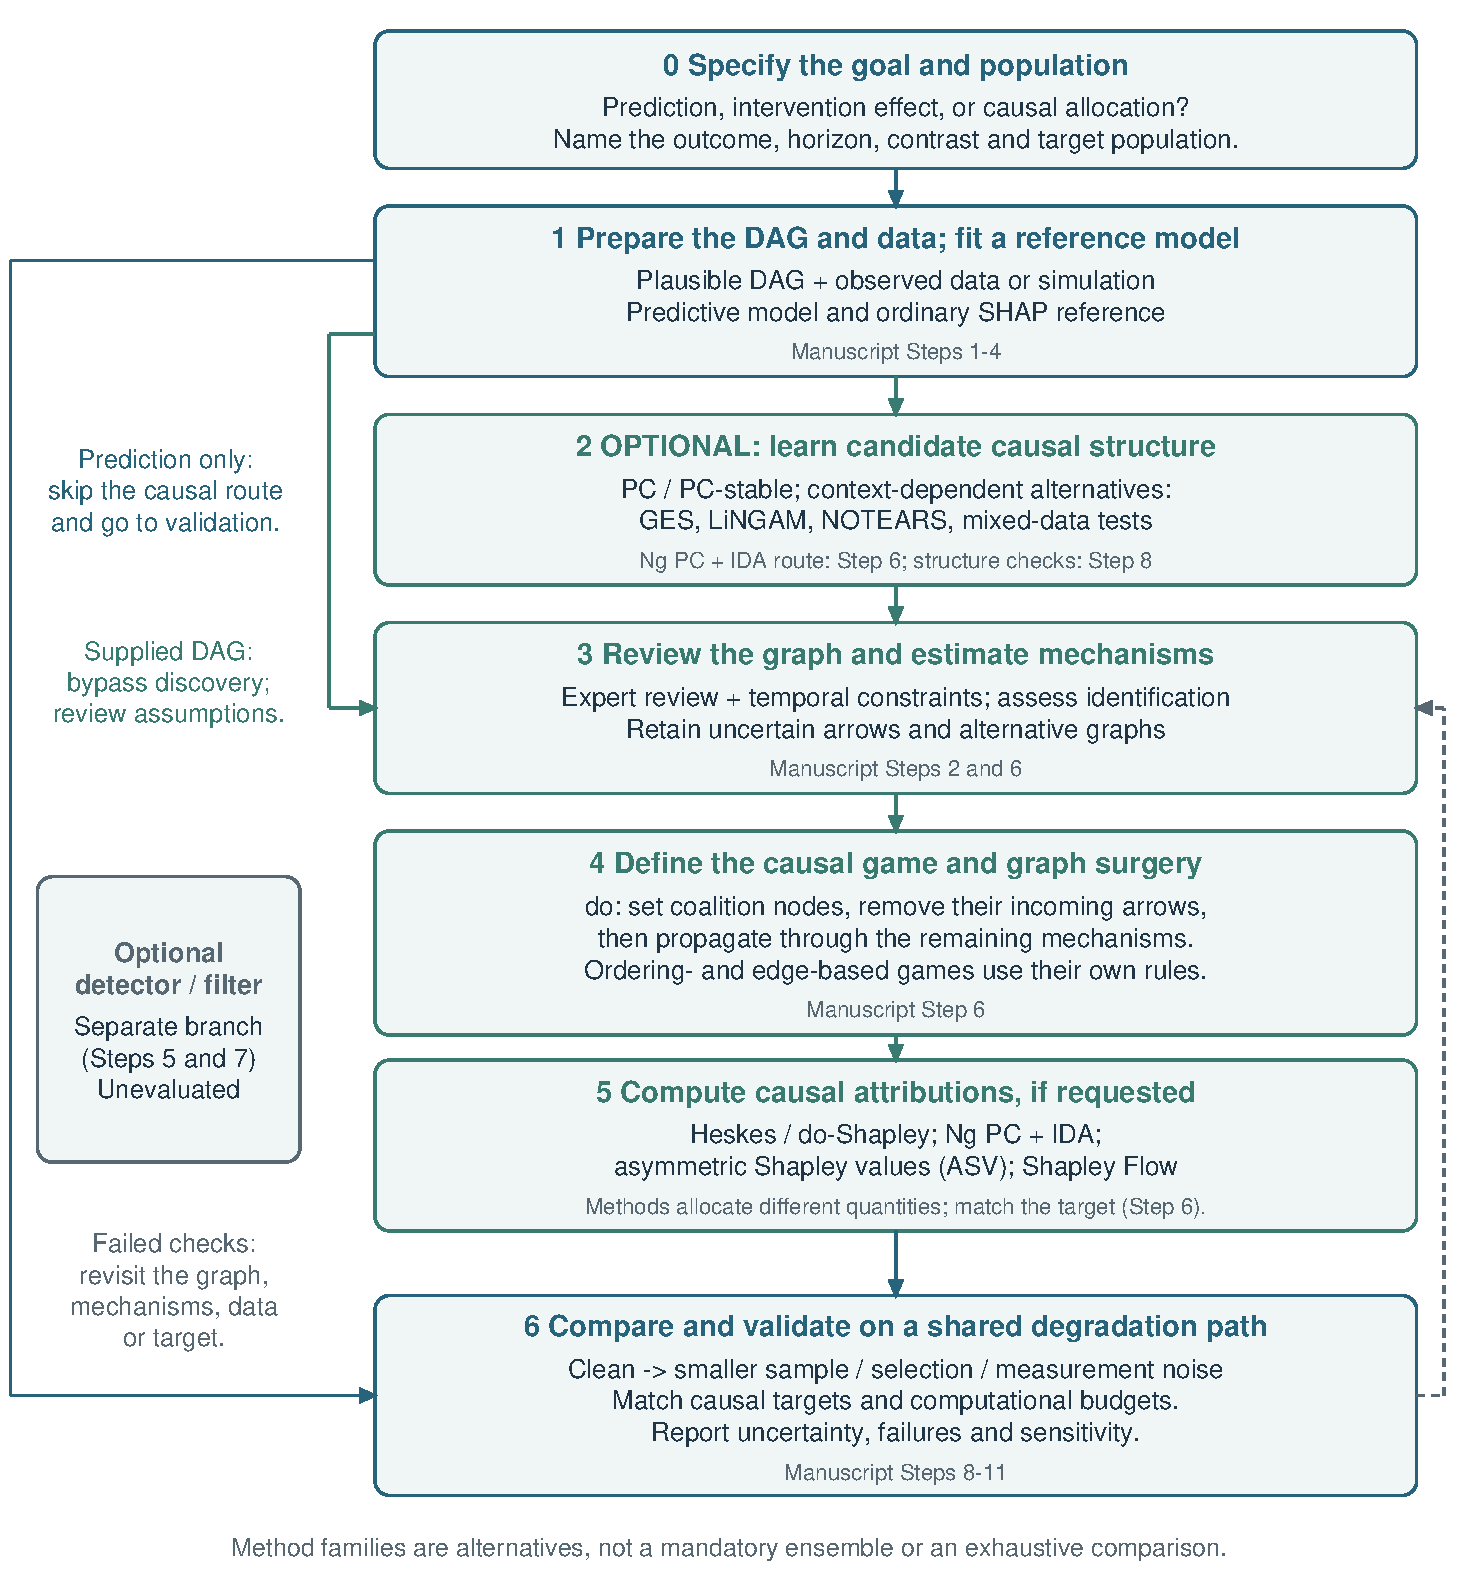
\includegraphics[width=\linewidth,height=0.68\textheight,keepaspectratio]{figures/method-workflow.pdf}
\captionof{figure}{The manuscript's methods grouped into seven stages (0--6). Discovery has a supplied-graph bypass. The predictive reference reaches evaluation directly; optional detector work remains unevaluated.}
\label{fig:workflow}
\end{center}

\clearpage
\section*{How the playbook maps to the manuscript}

The stage numbers below group the existing protocol; they do not replace its step numbers or imply that every method follows the same implementation. The manuscript's Step~6 contains several operations that are separated here so the reader can see where causal information enters.

\begingroup\small\setlength{\tabcolsep}{5pt}
\begin{longtable}{@{}L{0.27\linewidth}L{0.48\linewidth}L{0.18\linewidth}@{}}
\toprule Stage & Operation and output & Manuscript steps\\\midrule\endhead
0. Set the goal & Choose prediction, an intervention effect, or allocation of a joint contrast; specify population and timing. & 1; target definitions\\[5pt]
1. Prepare data and the predictive reference & Specify the plausible DAG and simulation mechanisms; generate data; fit a model and ordinary SHAP comparator. & 2--4\\[5pt]
2. Discover candidate structures (optional) & Run PC or a justified alternative; retain a partially directed graph where directions are unresolved. & Discovery in 6; comparison in 8\\[5pt]
3. Review the graph and estimate mechanisms & Use temporal and domain knowledge to assess edges, retain alternatives and fit the mechanisms required by the method. & 2; review in 6\\[5pt]
4. Define the causal game and graph surgery & Specify interventions, players, background and scale. For a do-game, replace intervened mechanisms and identify or propagate the resulting distribution. & Value-function part of 6\\[5pt]
5. Calculate causal attributions & Apply the selected node-, order-, weight- or edge-based allocation rule. & Attribution in 6\\[5pt]
6. Compare under data degradation & Evaluate the appropriate targets, repeat selected analyses under changed data conditions, and report uncertainty and limits. & 4, 6, 8; robustness 9--11\\
\bottomrule
\end{longtable}\endgroup

\textbf{Two playbooks through this sequence.} Prediction uses the fitted model and ordinary attribution from Stage~1, then predictive validation in Stage~6. The causal-attribution comparison proceeds through Stages~2--5, skipping discovery when a supplied graph is sufficient. An intervention-effect question needs the causal assumptions and effect calculation, but can omit Shapley allocation altogether. Ordinary SHAP is the study's comparator, not a prerequisite for every causal analysis.

The proposed detector can inspect the predictive or causal-attribution analysis (protocol Steps~5 and~7) and flag candidates for review. It is a separate research component, not an established repair. Longitudinal analysis (Step~12) and cost-constrained recourse (Step~13) remain extensions beyond the completed work.

\clearpage
\section*{Stages 0--1: goal, data and predictive reference}

\textbf{Stage 0.} Specify the quantity before selecting a method. The manuscript's primary exposure is cumulative mission duration and its outcome is nephrolithiasis. A risk forecast, a high-versus-low mission-duration effect and an allocation of a joint intervention contrast are different targets. A hydration-policy contrast can be a separate worked intervention, with its own timing and comparator. Harrell's purposes are hypothesis testing, estimation and prediction; modeling supports all three \citep{HarrellRMSIntroduction}. The prediction/intervention distinction concerns the claim we need to make \citep{HernanHsuHealy2019}.

\textbf{Stage 1.} Use the supplied renal topology to define a plausible system, then state the numerical mechanisms used to generate data. Keep the 14-node working subgraph and 51-node source DAG separate. For a blinded discovery comparison, hold the generating graph and reference quantities apart from the data given to the algorithm. An oracle-assisted calculation may use them, but must be labeled accordingly.

Fit the predictive reference on those data and compute ordinary SHAP with its background distribution and output scale stated. The existing study includes random forest and XGBoost TreeSHAP, logistic-regression LinearExplainer, and model-agnostic explanations. A prespecified regression is a useful reference; additional model flexibility is conditional on sample size and response shape. A mediator receiving large predictive credit can be correct for prediction even when an upstream intervention changes the outcome.

\section*{Stage 2: optional causal discovery}

\textbf{PC is the concrete starting point in this study}, including the discovery component of Ng et al.'s Causal SHAP. PC removes edges using conditional-independence tests and orients those justified by its rules; it generally returns a CPDAG, representing an equivalence class rather than a unique causal DAG \citep{Kalisch2012,Ng2025}. Under the usual formulation, causal sufficiency, acyclicity, Markov and faithfulness assumptions matter. A supplied graph can bypass this stage and enter graph review directly.

\begingroup\small\setlength{\tabcolsep}{5pt}
\begin{longtable}{@{}L{0.25\linewidth}L{0.69\linewidth}@{}}
\toprule Starting point or alternative & What changes, and why it might be appropriate\\\midrule\endhead
PC / PC-stable & PC-stable reduces order dependence in skeleton estimation. Choose tests suitable for the variable types; Gaussian tests are not a universal choice for the mixed renal data \citep{ColomboMaathuis2014}.\\[4pt]
GES & A score-based comparison when its model and score assumptions are justified \citep{Chickering2002}.\\[4pt]
LiNGAM & Uses functional assumptions such as linearity and non-Gaussian disturbances to identify directions \citep{Shimizu2006}.\\[4pt]
NOTEARS & A continuous-optimization alternative whose loss and model class must suit the data \citep{Zheng2018}.\\
\bottomrule
\end{longtable}\endgroup

The mixed-data test choice belongs inside the discovery comparison. Algorithm names alone do not establish suitability. The observed disconnected-outcome PC result is retained as a diagnostic; it is not justification for silently adding an outcome edge.

\clearpage
\section*{Stage 3: review the graph and estimate mechanisms}

Review candidate or supplied graphs against timing, biological evidence and the intended intervention. Record why each edge is retained, removed or oriented, and keep competing graphs when the evidence does not resolve them. Check whether their differences change identification of the target, not only whether their pictures look similar. The existing M1--M5 evaluation separates structural agreement from adjustment-set sufficiency and target-effect consequences.

\textbf{Reference comparison:} unrevised graph versus a documented revision under the same downstream method. \textbf{Conditional choice:} domain-informed review with an explicit ledger and retained uncertainty. For the intervention-propagation route, fit the required conditional mechanisms under the causal and identification assumptions of the chosen method, or declare that simulation mechanisms are supplied. A DAG specifies structure; it does not supply all functional forms or coefficients.

\section*{Stage 4: define interventions and perform graph surgery}

Graph review changes our hypothesis about the observational system. \emph{Graph surgery} instead represents a specified intervention on that system: replace the assignment equation of each intervened node by its imposed value and remove its incoming arrows. Keep the remaining mechanisms and propagate their consequences. This is the do-operator construction, not another discovery algorithm \citep{HernanRobins2020}.

\begin{center}
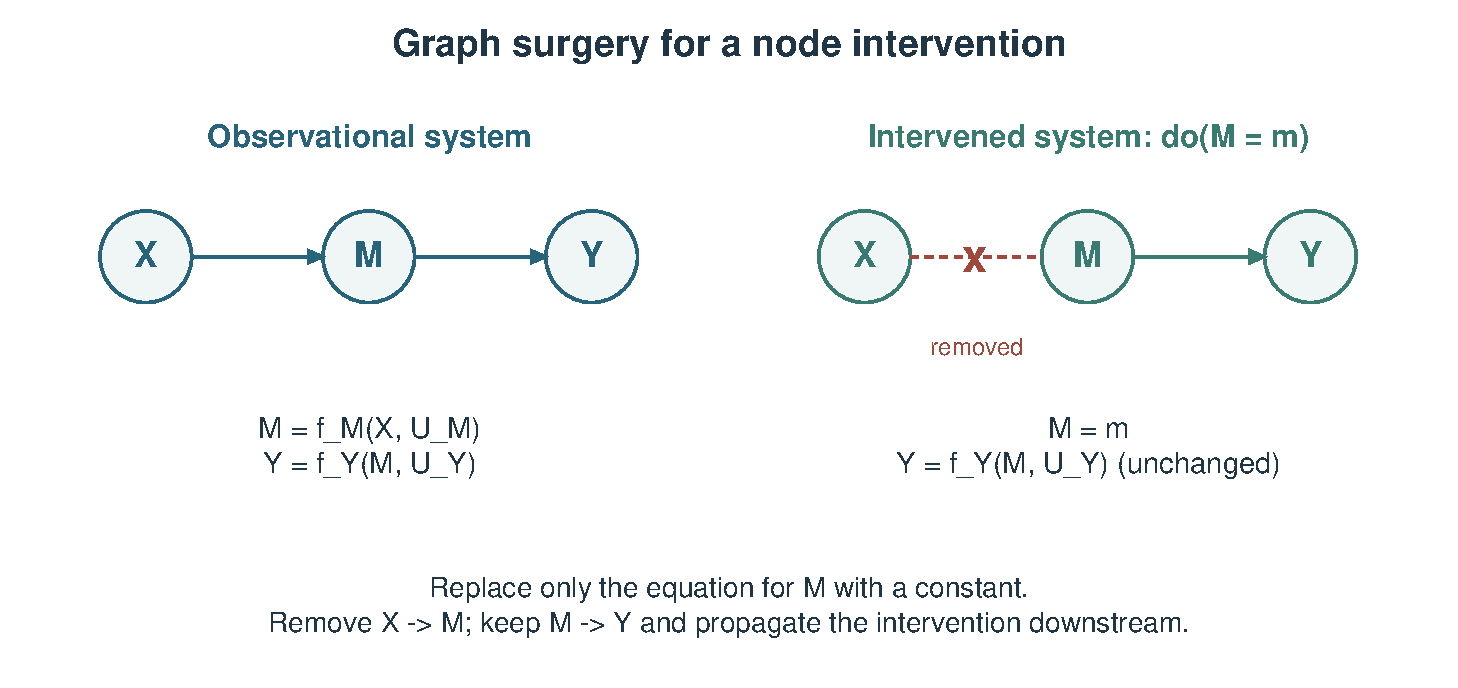
\includegraphics[width=\linewidth,height=0.20\textheight,keepaspectratio]{figures/graph-surgery.pdf}
\captionof{figure}{For $\dox(M=m)$ in a simple $X\to M\to Y$ chain, remove the incoming $X\to M$ arrow and replace the equation for $M$. The outgoing $M\to Y$ path remains. Observing $M=m$ does not perform this operation.}
\end{center}

For a coalition $C$, declare whether the value is an expected outcome or a model output:
\[
 v_Y(C)=\mathbb{E}[Y\mid\dox(X_C=x_C)],\qquad
 v_f(C)=\mathbb{E}[f(X)\mid\dox(X_C=x_C)].
\]
The two are not generally equal. The renal propagation prototype uses a fitted model output; outcome-based do-Shapley addresses a different declared game \citep{Heskes2020,Jung2022}.

In a causally sufficient, correctly specified DAG model, the post-intervention distribution can be obtained by retaining the factors for nonintervened nodes and fixing the coalition values. With observed data, identification, measurement and support must justify estimation; a drawn surgery alone does not identify an effect. Standardization or another identified estimator may replace explicit simulation when appropriate.

\textbf{Reference comparison:} an ordinary predictive coalition construction versus the explicitly declared interventional game. \textbf{Conditional choice:} use the latter when the target is causal allocation and its quantities are identifiable. ASV ordering and Shapley Flow have their own rules; they must not be relabeled as the same do-surgery calculation.

\clearpage
\section*{Stage 5: calculate method-specific causal attributions}

Once the value function and allocation rule are fixed, compute the contributions. For a symmetric Shapley game with player set $N$,
\[
 \phi_i(v)=\sum_{C\subseteq N\setminus\{i\}}
 \frac{|C|!(|N|-|C|-1)!}{|N|!}
 \bigl[v(C\cup\{i\})-v(C)\bigr].
\]
Changing the value function, permitted orders, players, background, output scale or aggregation changes what is being attributed. The methods in protocol Step~6 therefore occupy the same comparison stage without becoming interchangeable implementations.

\begingroup\small\setlength{\tabcolsep}{5pt}
\begin{longtable}{@{}L{0.27\linewidth}L{0.67\linewidth}@{}}
\toprule Method & Information supplied and operation\\\midrule\endhead
Causal Shapley / do-Shapley & Evaluate specified interventional coalition quantities and allocate their increments. Distinguish model-output games from outcome-based games; the latter are the focus of Jung et al. \citep{Heskes2020,Jung2022}.\\[5pt]
Ng et al. Causal SHAP & Uses PC-derived structure, IDA causal-strength information and a weighted, normalized attribution construction. It is not automatically the symmetric outcome do-Shapley game \citep{Ng2025}.\\[5pt]
Asymmetric Shapley values (ASV) & Incorporate causal ordering through the order weights. Ordering alone does not add a mechanism for downstream intervention propagation \citep{Frye2020}.\\[5pt]
Shapley Flow & Allocates credit to graph edges, with the explanation boundary stated. Its edge scores are a different object from node-level outcome effects \citep{Wang2021}.\\
\bottomrule
\end{longtable}\endgroup

\textbf{Reference comparison:} ordinary SHAP and the manuscript's selected causal variants, with their information inputs visible. \textbf{Conditional choice:} choose the family that matches the scientific target and the causal information available. There is no unconditional winner or verified ``most cited'' ranking in this guide.

For the renal study, three causal methods have run on the working subgraph. The Heskes-style working-subgraph route was blocked; the separate full-DAG propagation prototype receives known simulation mechanisms and uses graph-respecting orders. It is an oracle-mechanism calculation, not evidence that those mechanisms were learned from sparse observational data.

An interventional Shapley allocation shares its specified joint contrast among players. It need not equal the effect of intervening on one player. If the question is simply the effect of one feasible intervention, report that contrast without requiring a Shapley decomposition. Action selection additionally needs feasibility, harms, costs and preferences.

\clearpage
\section*{Stage 6: compare on a common degradation path}

The common experimental axis is to rerun selected method comparisons as data move from a clean simulated setting toward the constraints of spaceflight cohorts. This follows the collaborators' proposed analysis arc; the systematic degradation experiment is not yet a completed result.

\begingroup\small\setlength{\tabcolsep}{5pt}
\begin{longtable}{@{}L{0.25\linewidth}L{0.69\linewidth}@{}}
\toprule Change to the data & What to hold fixed and what to assess\\\midrule\endhead
Smaller samples & Keep mechanisms and targets fixed; refit the pipeline across seeds and report uncertainty and failures.\\[4pt]
Selection & Separate entry, assignment and recording. Distinguish a changed selected-population effect from estimation or transport error.\\[4pt]
Measurement error or missingness & Specify which nodes and mechanisms are affected; vary these separately before combining them. They are not equivalent to reducing sample size.\\[4pt]
Mechanism or population shift & Declare what changes and the target population. Nonlinear mechanisms and out-of-distribution settings need their own checks.\\
\bottomrule
\end{longtable}\endgroup

Report predictive performance, graph recovery, causal-attribution accuracy and intervention-ranking agreement separately. An accuracy oracle must match the method's actual game and allocation rule. Comparing every method to a common symmetric do-Shapley target is a target-agreement study when their estimands differ. Kendall's $\tau$ against individual intervention effects remains a separate screening-agreement diagnostic.

\textbf{Reference comparison:} the clean-data result with resampling. \textbf{Conditional choice:} prespecified degradation settings, repeated full-pipeline fits, matched information and computation budgets, and uncertainty tied to the claim. An evaluation-record bootstrap for one fitted model does not replace repeated training runs. Vary one consequential choice at a time where possible; the full grid of methods and settings is outside this study.

\textbf{Selection in the renal example.} Add eligibility $E$, mission assignment $G$ and recording $R$ alongside the biological DAG. For hydration assigned after selection, an effect among eligible assigned crew need not equal an effect in a broader source population. Weighting requires measured relevant variables, transport assumptions and support; it cannot create an absent subgroup. The existing selection overlay and exact illustrative calculation remain companion material, not new renal results.

\textbf{Current evidence.} Credit shifts vary by model and pathway. The matched full-DAG ordering comparison found no detected improvement; the separate propagation prototype uses more causal information and a different budget. Working-subgraph revision rounds two and three are scripted heuristics. Human expert review, the detector, matched-game renal attribution oracles and the broader robustness comparison remain unfinished.

\textbf{Scope.} Keep the detector/filter as an optional, explicitly unevaluated branch. A planted mediation example can define a future detector test; it does not establish universal suppression of upstream causes. Educator-companion development is paused. The technical note and method appendix retain the fuller derivations and alternatives.

\clearpage
\small
\bibliographystyle{unsrtnat}
\bibliography{references}
\end{document}
